\section{Interférences}

Le phénomène d'interférence est du à la superposition de deux
ondes.

Il en résulte des zones où les ondes s'additionnent (zone de
tempête) et des zones où la superposition des ondes donne une amplitude
résultante nulle (zone de repos).

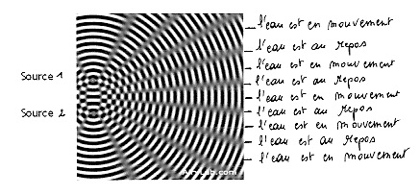
\includegraphics[width=8.326cm,height=3.881cm]{Pictures/10000001000001A4000000C3DDA5D7BD0B699726.png}

\subsection{Expérience avec la cuve à onde}

FIXME ajouter des descriptions d'expériences avec la cuve à ondes

Nous avons visualisé ce phénomène à l'aide de la cuve à ondes.

Pour ce faire, nous avons pris des pointes qui vibrent dans l'eau,
chacune produisant des ondes circulaires.

Nous avons obervé des endroits où l'eau est en mouvement et des endroits
où l'eau est au repos. Comment expliquer cette observation?

\subsubsection{Analyse théorique}

Prenons deux sources $S_1$ et $S_2$ émettant
en concordance de phase des ondes de même fréquence (on dira que les
sources sont alors \emph{cohérentes}).

\begin{figure}
\centering
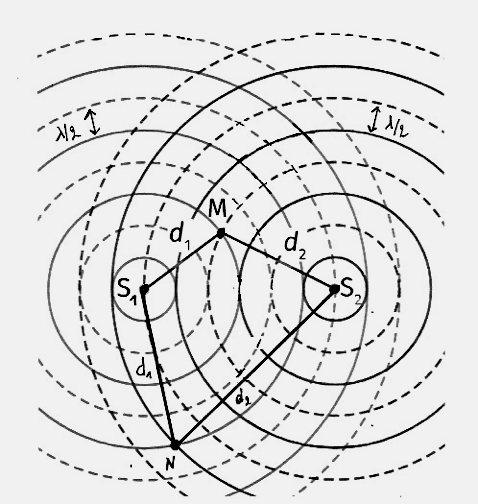
\includegraphics[width=8.47cm,height=8.927cm]{Pictures/10000001000001DE000001F885F9EB969C92123B.png}
\caption{}
\end{figure}

Les cercles concentriques représentent les vagues vues de haut
\emph{(les cercles en traits pleins des crètes et les cercles en traits
pointillés des creux).}

Nous voyons bien que les 2 sources ($S_{1}$ et
$S__{2}$) émettent des ondes de même longueur d'onde et donc
de même fréquence.

Considérons le point M. 

L'onde produite par $S_1$ a parcouru une distance
$d_1$ pour arriver en M et l'onde produite par
$S_2$ a parcouru une distance $d_2$ pour
arriver en M. Les deux ondes arrivent donc au point M avec un déphasage
puisqu'elle n'ont pas parcouru la même distance.

Dans notre exemple ci-contre :
\begin{enumerate}
	\item La distance $d_1$ parcourue par l'onde provenant de
	$S_1$ jusque M est égale à $3 \cdot \frac{1}{2}$ (trois demi-longueur
	d'onde). Regardez sur le schéma.
	\item La distance $d_2$ parcourue par l'onde provenant de
	$S_2$} jusque M est égale à $4 \cdot \frac{1}{2}$(quatre demi-longueur
	d'onde).
	\item  Les deux ondes arrivent donc en M décalées de $\frac{4}{2} - \frac{3}{2} = \frac{1}{2} $
\end{enumerate}

Elles sont donc au point M en opposition de phase l'une par rapport à
l'autre. En effet, au point M, l'onde provenant de $S_1$
est une crète tandis que l'onde provenant de $S_2$ est un
creux. Donc, au point M, l'eau sera au repos. On parlera
\emph{d'interférence destructive.}

Nous appelerons \textbf{$d_2 - d_1 = \Delta_{12}, \emph{la différence de
marche.}

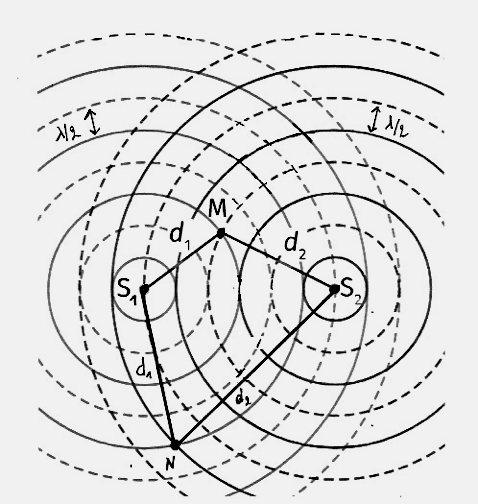
\includegraphics[width=9.596cm,height=10.112cm]{Pictures/10000001000001DE000001F885F9EB969C92123B.png}

Considérons le point N. 

L'onde produite par $S_1$ a parcouru une distance
d\textsubscript{1} pour arriver en N et l'onde produite par
$S_2$ a parcouru une distance d\textsubscript{2} pour
arriver en N. Les deux ondes arrivent donc au point M avec un déphasage.
\begin{enumerate}
	\item La distance $d_1$ parcourue par l'onde provenant de
	$S_1$ jusque M est égale à $5 \frac{1}{2}$ (cinq demi-longueur
	d'onde). Regardez sur le schéma.
	\item La distance $d_2$ parcourue par l'onde provenant de
	$S_2$ jusque N est égale à $75 \frac{1}{2}$ (sept demi-longueur
	d'onde).
	\item Les deux ondes arrivent donc en M décalées de ($\frac{7}{2} - \frac{5}{2} =  \frac{2}{2}$ longueur d'ondes.
\end{enumerate}

Elles sont donc au point N en concordance de phase l'une par rapport à
l'autre. En effet, au point N, l'onde provenant de $S_1$
est une crète et de même, l'onde provenant de $S_2$ est une
crète. Donc, au point N, deux crètes vont se superposer, ce qui donnera
de l'eau en mouvement avec une amplitude double par rapport aux
amplitudes des sources. On parlera \emph{\textbf{d'interférence
constructive.}}

\emph{\textbf{ }}

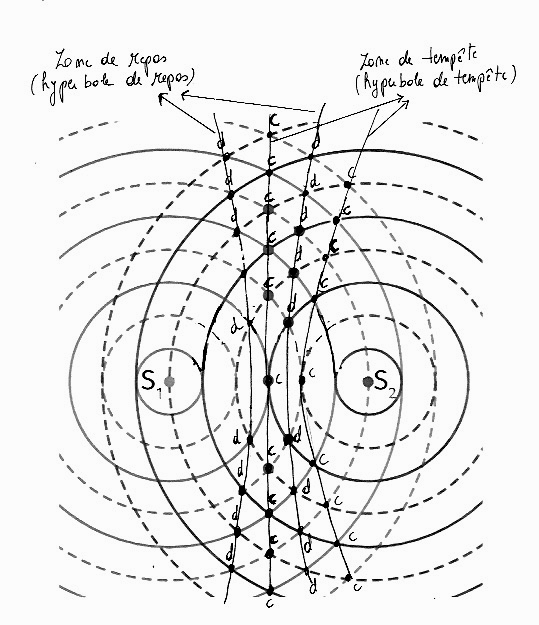
\includegraphics[width=7.264cm,height=8.423cm]{Pictures/100000010000021B000002719784CD0CAF081F55.png}\emph{\textbf{Hyperboles
de repos et hyperboles de tempête}}

Pour expliquer les zones de tempête et de repos, observez attentivement
le schéma ci-contre :

\emph{1) En chaque point d :}

Chaque point d est atteint par un creux (cercle en pointillé)
\emph{\textbf{et}} une crète (cercle en trait plein), la résultante du
mouvement nous donne donc une \textbf{zone de repos.} Vous pouvez ainsi
observer ces courbes (ce sont des hyperboles) où l'eau au repos.

\emph{2) En chaque point c : }

Chaque point c est atteint par soit deux creux (cercles en pointillé) ,
soit deux crètes (cercles en trait plein), la résultante du mouvement
nous donne donc une \textbf{zone de tempête.} Vous pouvez ainsi observer
ces courbes (ce sont des hyperboles) où l'eau est en mouvement.

\begin{figure}
\centering
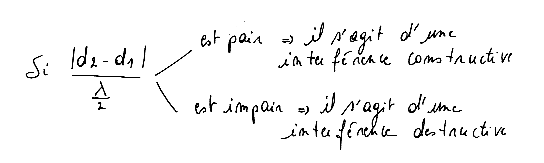
\includegraphics[width=13.005cm,height=3.542cm]{Pictures/1000000100000220000000A31734CD7DA5F285B4.png}
\caption{}
\end{figure}

\emph{\textbf{EXERCICE 1}}

Soient deux sources sonores ponctuelles S1 et S2. Elles envoient des
ondes en concordance de phase, dont la fréquence est égale à 5 Hz et qui
se propagent à la vitesse de 10 cm/s. L'amplitude de chacune des ondes
est de 3cm

Calculez l'amplitude d'un point P situé à 6 cm de S1 et à 8 cm de S2~?

\emph{\textbf{EXERCICE 2}}

Deux haut-parleurs séparés de 2 m émettent un signal à 680 Hz en phase.
Un microphone est placé à 6,75 m de l'un et à 7 m de l'autre. Quelle est
l'amplitude du signal mesuré~?

\emph{\textbf{EXERCICE 3}}

\begin{figure}
\centering
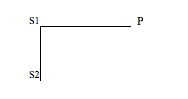
\includegraphics[width=5.151cm,height=2.729cm]{Pictures/10000001000000BC000000630AF71C86AA2A0A65.png}
\caption{}
\end{figure}

Deux haut-parleurs S1 et S2 distants de 6 m émettent des

ondes sonores en concordance de phase. Le point P de la

figure est à 8 m de S1. Quelle est la fréquence minimale

à laquelle l'intensité en P est~:

\begin{enumerate}
\def\labelenumi{\alph{enumi})}
\tightlist
\item
  nulle~?
\end{enumerate}

\begin{enumerate}
\def\labelenumi{\alph{enumi})}
\tightlist
\item
  maximale~?
\end{enumerate}

\emph{\textbf{EXERCICE 4}}

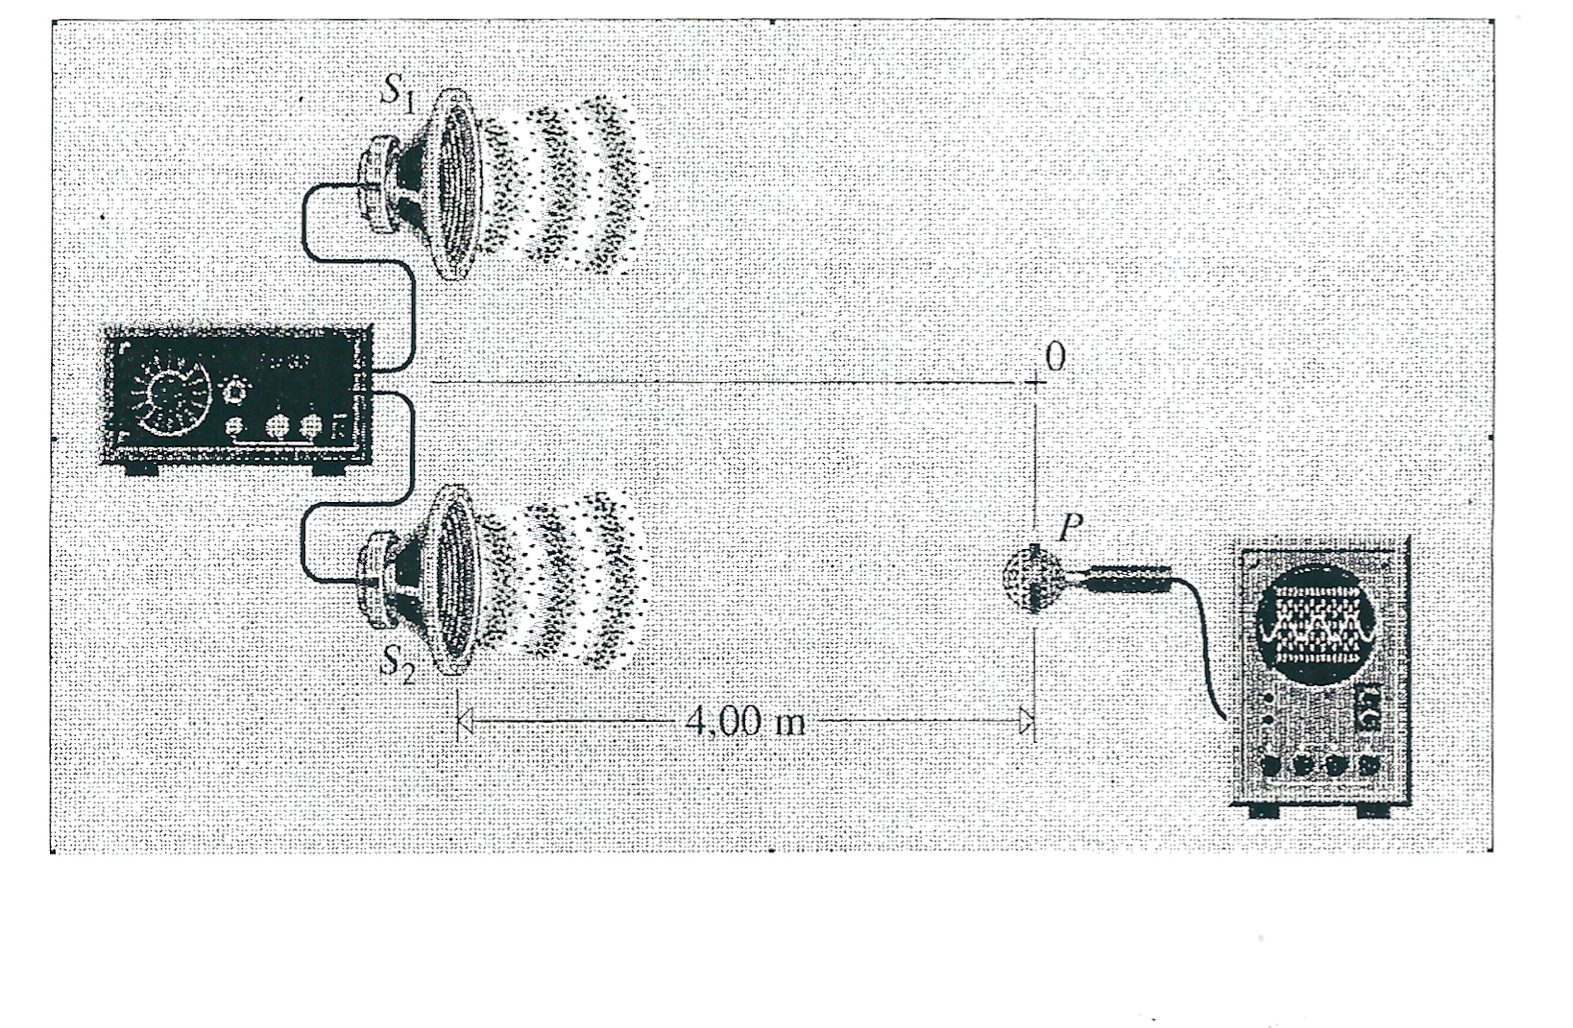
\includegraphics[width=9.146cm,height=5.973cm]{Pictures/100000010000062500000404B4675BF2C4CE1EEC.png}Deux
petits haut-parleurs distants de 3 mètres émettent des sons de fréquence
constante de 344 Hz dans une pièce surchauffée. On déplace un microphone
P le long d'une droite parallèle à la ligne S1S2 joignant les deux
haut-parleurs et située à 4 mètres de cette ligne. On trouve deux maxima
d'intensité~: le premier au point O, équidistants des deux haut-parleurs
et le second juste en face de l'un d'eux.

Utilisant ces données, calculer la vitesse du son dans cette pièce
surchauffée

( rappel~: la vitesse du son dans l'air est de 340 m/s à une température
de 20°C)

\emph{\textbf{EXERCICE 5}}

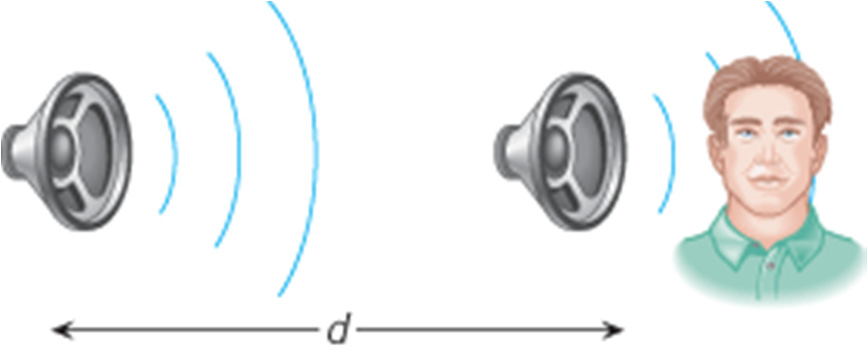
\includegraphics[width=11.546cm,height=4.688cm]{Pictures/1000000100000363000001603D3E7105AB252F90.png}Les
deux haut-parleurs montrés sur la figure émettent, en phase, un son
ayant une longueur d'onde de 25 cm. Quelle est la distance minimale d
entre les haut-parleurs qu'il doit y avoir pour qu'il y ait de
l'interférence destructive pour l'observateur?

\emph{\textbf{EXERCICE 6}}

\begin{figure}
\centering
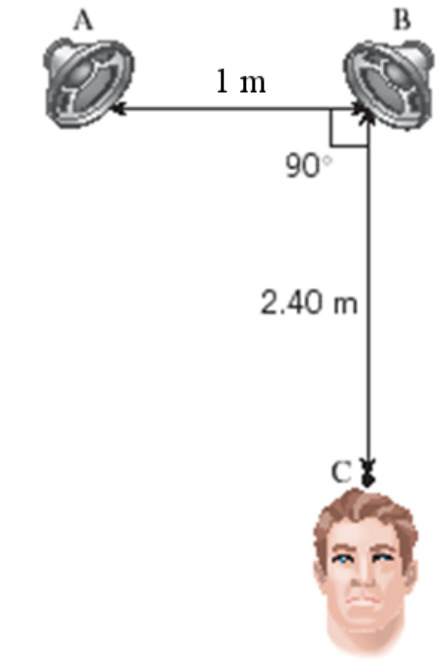
\includegraphics[width=4.757cm,height=7.147cm]{Pictures/10000001000001BA00000298E2F6E319C348E061.png}
\caption{}
\end{figure}

Les haut-parleurs de la figure émettent des ondes sonores en concordance
de phase. Quelle est la fréquence minimale qui permet d'obtenir de
l'interférence destructive à l'endroit où est situé l'observateur?

\emph{\textbf{INTERFERENCES - EXERCICES}}

\emph{\textbf{EXERCICE 1}}

Soient deux sources sonores ponctuelles S1 et S2. Elles envoient des
ondes en concordance de phase, dont la fréquence est égale à 5 Hz et qui
se propagent à la vitesse de 10 cm/s. L'amplitude de chacune des ondes
est de 3cm

Calculez l'amplitude d'un point P situé à 6 cm de S1 et à 8 cm de S2~?

\emph{\textbf{EXERCICE 2}}

Deux haut-parleurs séparés de 2 m émettent un signal à 680 Hz en phase.
Un microphone est placé à 6,75 m de l'un et à 7 m de l'autre. Quelle est
l'amplitude du signal mesuré~?

\emph{\textbf{EXERCICE 3}}

\begin{figure}
\centering
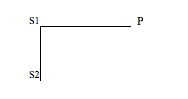
\includegraphics[width=5.151cm,height=2.729cm]{Pictures/10000001000000BC000000630AF71C86AA2A0A65.png}
\caption{}
\end{figure}

Deux haut-parleurs S1 et S2 distants de 6 m émettent des

ondes sonores en concordance de phase. Le point P de la

figure est à 8 m de S1. Quelle est la fréquence minimale

à laquelle l'intensité en P est~:

\begin{enumerate}
\def\labelenumi{\alph{enumi})}
\tightlist
\item
  nulle~?
\end{enumerate}

\begin{enumerate}
\def\labelenumi{\alph{enumi})}
\tightlist
\item
  maximale~?
\end{enumerate}

\emph{\textbf{EXERCICE 4}}

Deux petits haut-parleurs distants de 3 mètres émettent des sons de
fréquence constante de 344 Hz dans une pièce surchauffée. On déplace un
microphone P le long d'une droite parallèle à la ligne S1S2 joignant les
deux haut-parleurs et située à 4 mètres de cette ligne. On trouve deux
maxima d'intensité~: le premier au point O, équidistants des deux
haut-parleurs et le second juste en face de l'un d'eux.

Utilisant ces données, calculer la vitesse du son dans cette pièce
surchauffée

( rappel~: la vitesse du son dans l'air est de 340 m/s à une température
de 20°C)

\begin{figure}
\centering
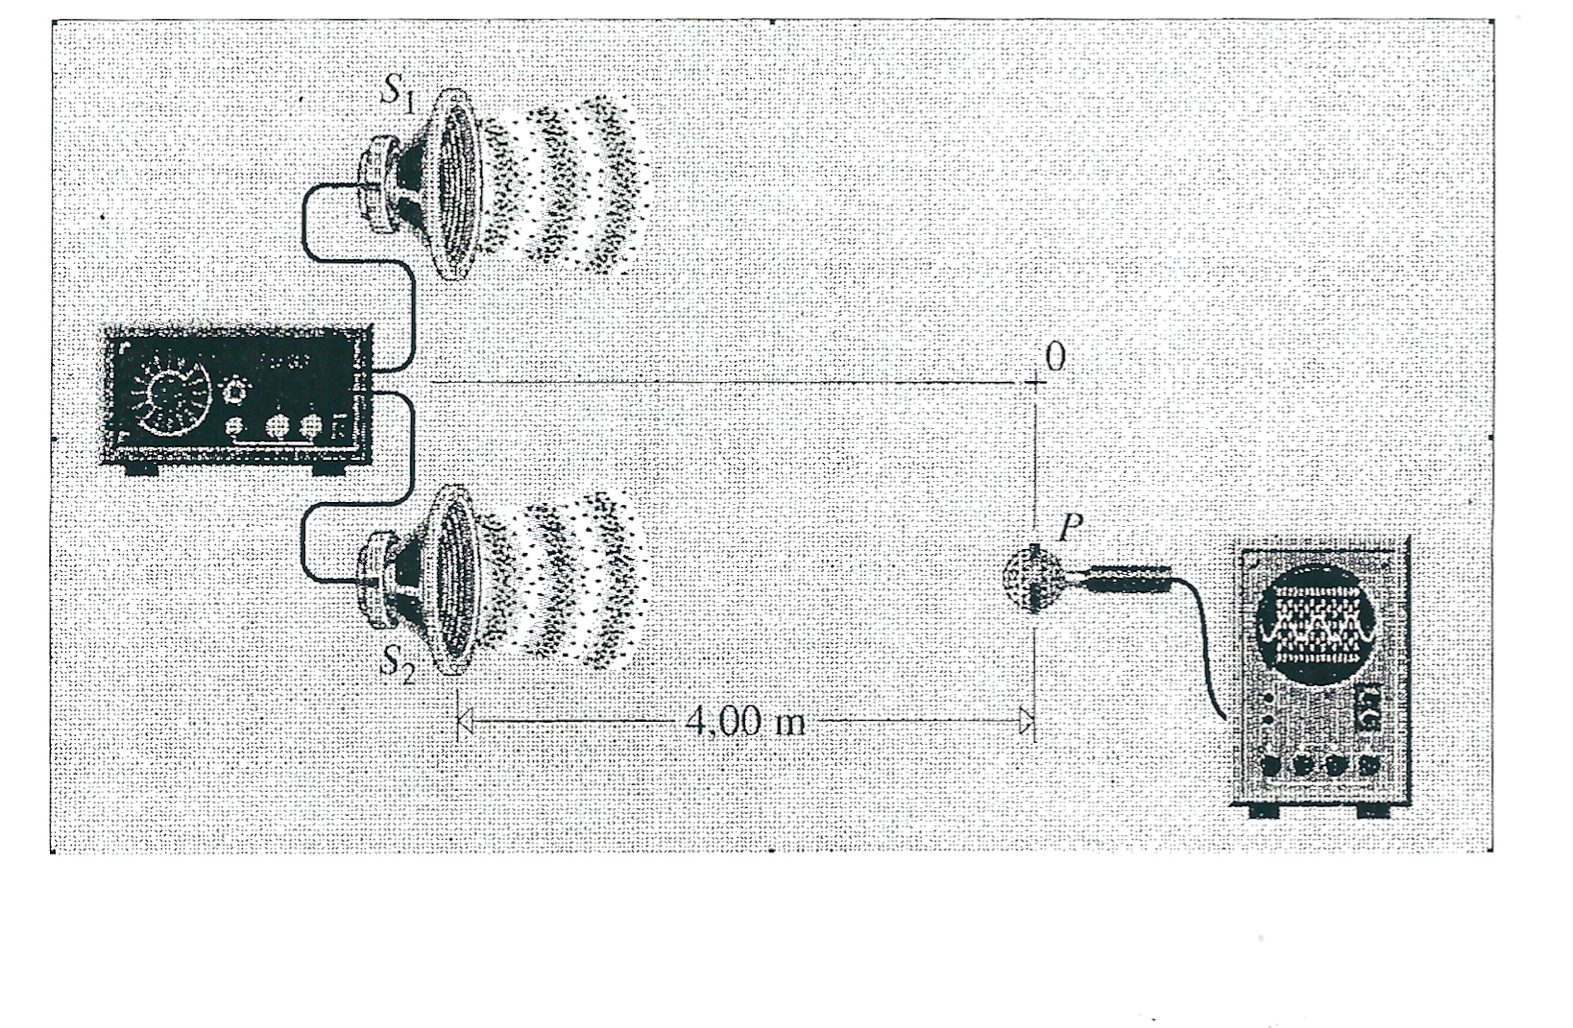
\includegraphics[width=15.663cm,height=10.231cm]{Pictures/100000010000062500000404B4675BF2C4CE1EEC.png}
\caption{}
\end{figure}

\emph{\textbf{EXERCICE 5}}

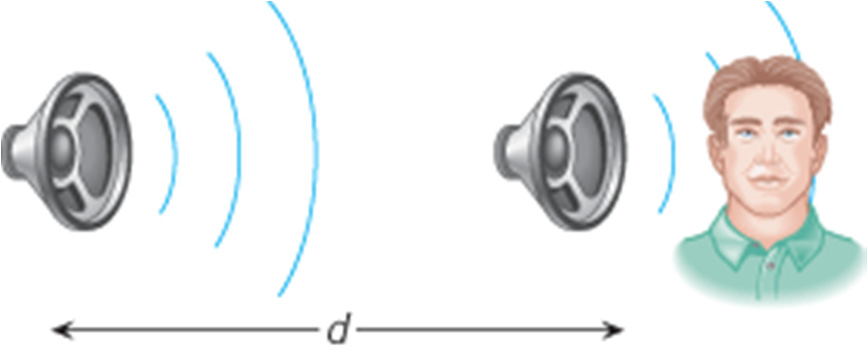
\includegraphics[width=11.546cm,height=4.688cm]{Pictures/1000000100000363000001603D3E7105AB252F90.png}Les
deux haut-parleurs montrés sur la figure émettent, en phase, un son
ayant une longueur d'onde de 25 cm. Quelle est la distance minimale d
entre les haut-parleurs qu'il doit y avoir pour qu'il y ait de
l'interférence destructive pour l'observateur?

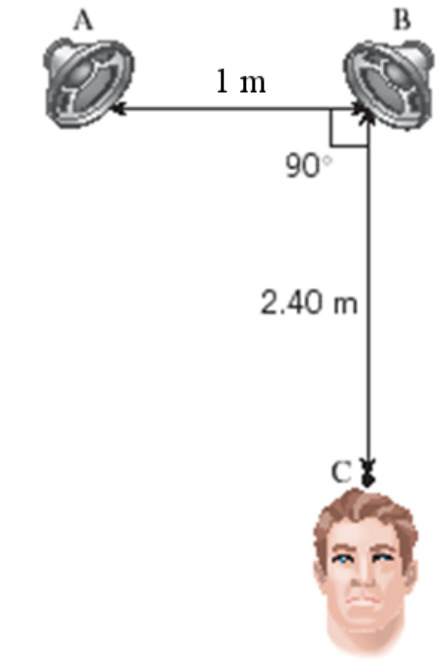
\includegraphics[width=4.757cm,height=7.147cm]{Pictures/10000001000001BA00000298E2F6E319C348E061.png}\emph{\textbf{EXERCICE
6}}

Les haut-parleurs de la figure émettent des ondes sonores en phase.
Quelle est la fréquence minimale qui permet d'obtenir de l'interférence
destructive à l'endroit où est situé l'observateur?

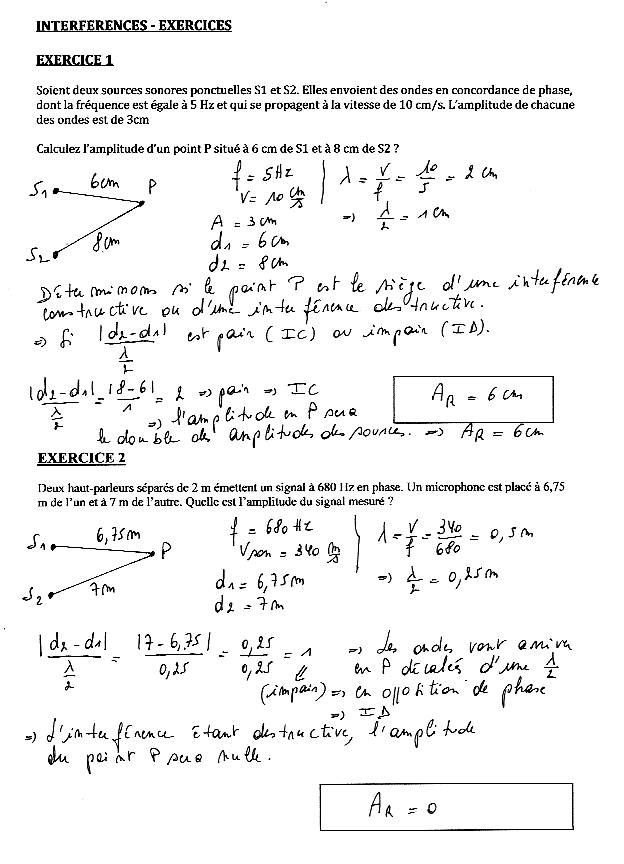
\includegraphics[width=18.253cm,height=25.273cm]{Pictures/100000010000027000000360A2E9B52B5C1C825B.png}

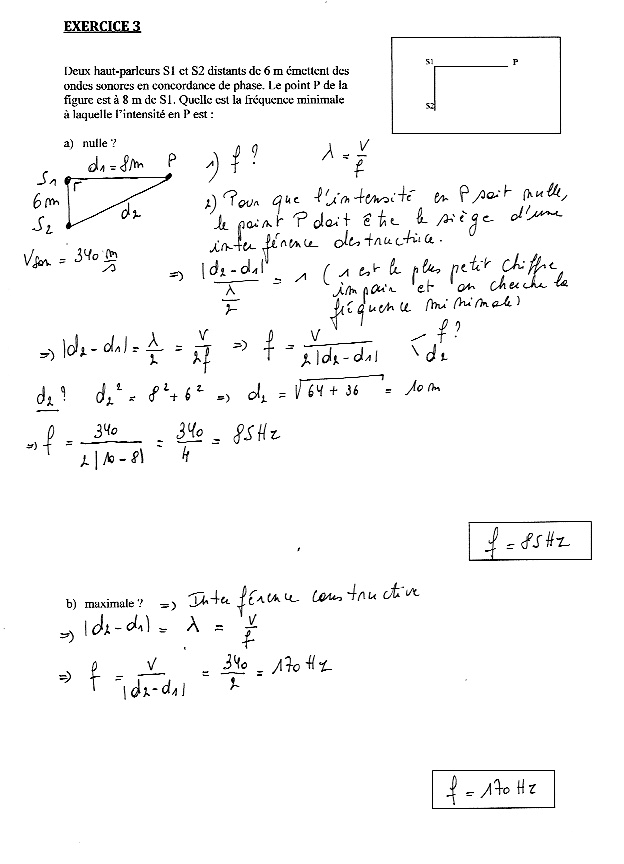
\includegraphics[width=18.253cm,height=25.273cm]{Pictures/100000010000027000000360F8FFC5B3763173F1.png}

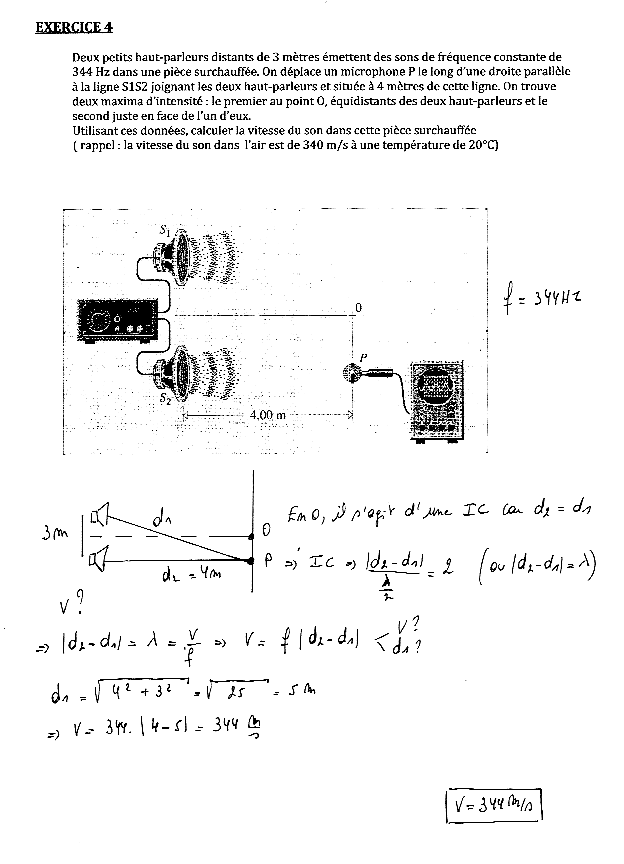
\includegraphics[width=18.253cm,height=25.273cm]{Pictures/100000010000027000000360FFD6C2C9381DA208.png}

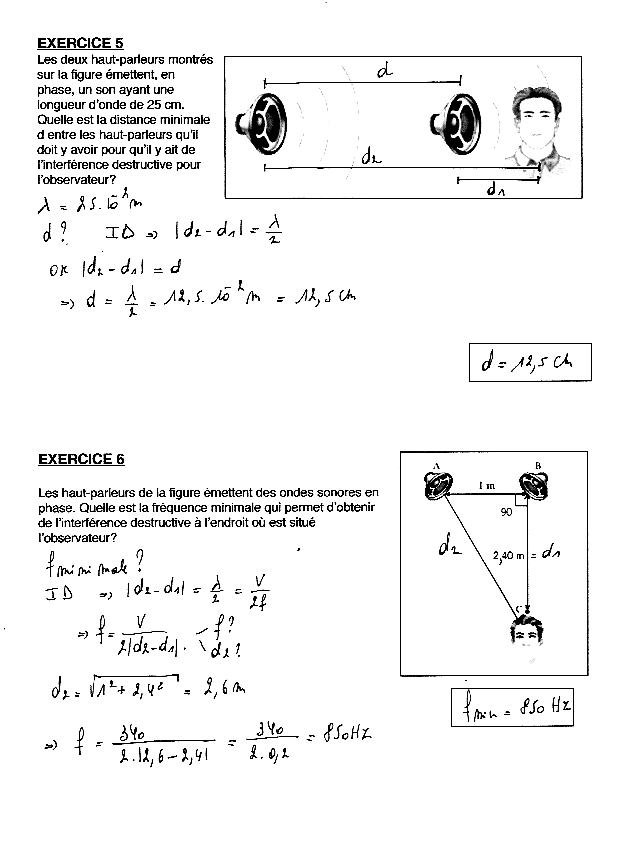
\includegraphics[width=18.253cm,height=25.273cm]{Pictures/1000000100000270000003604BA27A8CAE787E63.png}
